\chapter{Исследовательская часть}

В данном разделе будут приведены примеры работы программы, и будет проведен сравнительный анализ реализованных алгоритмов умножения матриц по затраченному процессорному времени.

\section{Технические характеристики}

Тестирование проводилось на устройстве со следующими техническими характеристиками:

\begin{itemize}
	\item операционная система Windows 10 pro;
	\item память 32 Гб;
	\item процессор Intel(R) Core(TM) i5-12400 12th Gen 2.50 ГГц.
\end{itemize}

Тестирование проводилось на компьютере, включенном в сеть электропитания. Во время тестирования компьютер был нагружен только встроенными приложениями окружения, а также непосредственно системой тестирования.

\clearpage

\section{Демонстрация работы программы}

На рисунке \ref{img:example} приведен пример работы программы.

\begin{figure}[H]
	\begin{center}
		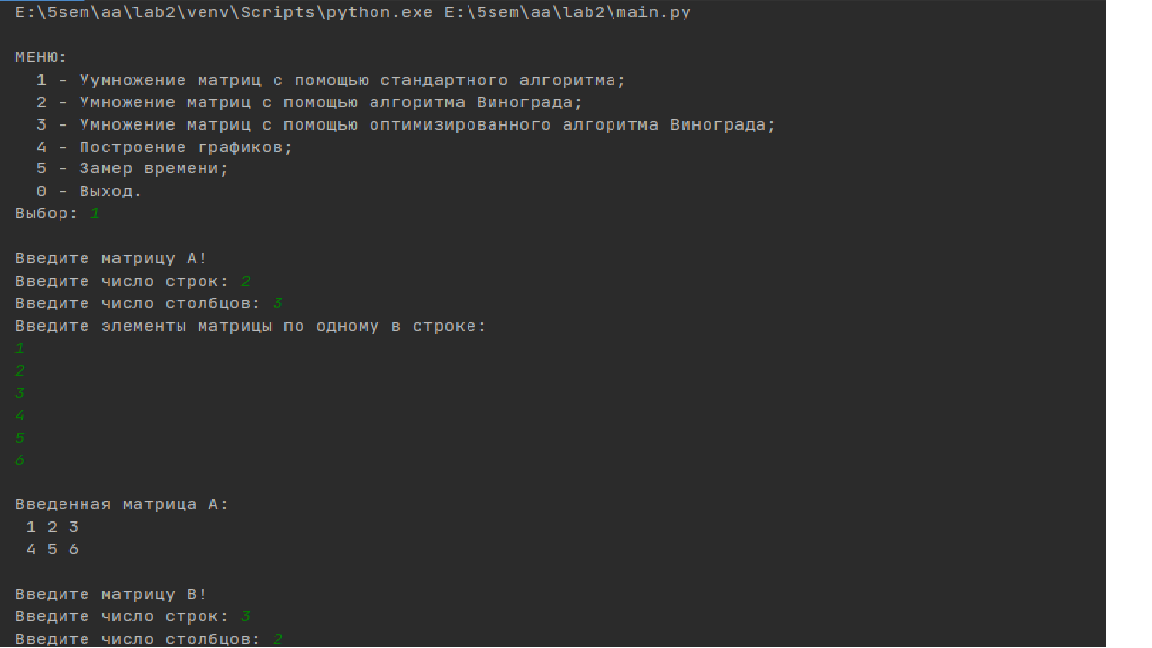
\includegraphics[scale=0.5]{img/example.png}
	\end{center}
	\captionsetup{justification=centering}
	\caption{Пример работы программы}
	\label{img:example}
\end{figure}

\section{Время выполнения алгоритмов}

Функция process\_time из библиотеки time языка программирования Python возвращает  процессорное время в секундах - значение типа float.

Для замера времени:
\begin{itemize}
	\item получить значение времени до начала выполнения алгоритма, затем после её окончания. Чтобы получить результат, необходимо вычесть из второго значения первое;
	\item первый шаг необходимо повторить iters раз (в программе iters равно 10), суммируя полученные значения, а затем усреднить результат.
\end{itemize}

Замеры проводились для квадратных матриц целых чисел, заполненных случайным образом, размером от 10 до 100 и от 11 до 101. Результаты измерения времени для четного размера матриц приведены в таблице \ref{tbl:time_even} (в мс).

\begin{table}[h]
    \begin{center}
        \begin{threeparttable}
        \captionsetup{justification=raggedright,singlelinecheck=off}
        \caption{Результаты замеров времени}
        \label{tbl:time_even}
        \begin{tabular}{|c|c|c|c|}
            \hline
            Размер & Стандартный (в мс) & Винограда (в мс) & Опт-ый Винограда (в мс)  \\
            \hline
		    10 & 0.2420 & 0.2235 & 0.1985 \\ 
		    \hline
		    20 & 1.7565 & 1.3610 & 1.4475 \\ 
		    \hline
		    30 & 3.1250 & 2.4730 & 2.5385 \\ 
		    \hline
		    40 & 4.8820 & 4.3975 & 4.2115 \\ 
		    \hline
		    50 & 10.9375 & 9.5350 & 7.8125 \\ 
		    \hline
		    60 & 17.1875 & 15.6250 & 14.0625 \\ 
		    \hline
		    70 & 29.6875 & 25.0000 & 21.8750 \\ 
		    \hline
		    80 & 43.7500 & 39.0625 & 32.8125 \\ 
		    \hline
		    90 & 57.8125 & 54.6875 & 46.8750 \\ 
		    \hline
		    100 & 78.1250 & 66.5270 & 62.5000 \\ 
		    \hline
		\end{tabular}
    \end{threeparttable}
\end{center}
\end{table}

На рисунке \ref{img:even} приведены графические результаты сравнения временных характеристик для четного размера матриц.

\begin{figure}[H]
	\begin{center}
		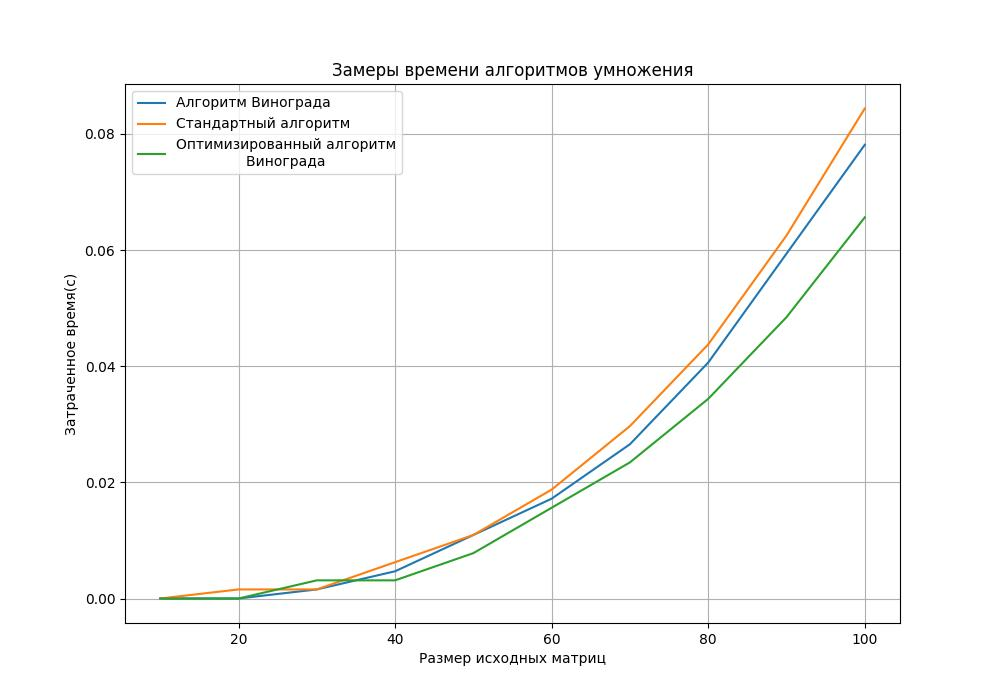
\includegraphics[scale=0.5]{img/even.jpeg}
	\end{center}
	\captionsetup{justification=centering}
	\caption{Сравнение по времени алгоритмов умножения матриц четного размера}
	\label{img:even}
\end{figure}

Результаты измерения времени для четного размера матриц приведены в таблице \ref{tbl:time_odd} (в мс).

\begin{table}[h]
    \begin{center}
        \begin{threeparttable}
        \captionsetup{justification=raggedright,singlelinecheck=off}
        \caption{Результаты замеров времени}
        \label{tbl:time_odd}
        \begin{tabular}{|c|c|c|c|}
            \hline
            Размер & Стандартный (в мс) & Винограда (в мс) & Опт-ый Винограда (в мс)  \\
            \hline
			   11 & 0.3450 & 0.5625 & 0.2785 \\ 
			\hline
			21 & 1.3655 & 0.9880 & 1.1695 \\ 
			\hline
			31 & 3.5330 & 3.1915 & 2.5625 \\ 
			\hline
			41 & 6.2500 & 5.1325 & 4.6875 \\ 
			\hline
			51 & 10.9375 & 9.9440 & 9.3750 \\ 
			\hline
			61 & 20.3125 & 17.1875 & 14.0625 \\ 
			\hline
			71 & 31.2500 & 26.5625 & 23.4375 \\ 
			\hline
			81 & 45.3125 & 37.0625 & 32.8125 \\ 
			\hline
			91 & 60.9375 & 58.6430 & 46.8750 \\ 
			\hline
			101 & 81.6875 & 79.6875 & 65.6250 \\ 
			\hline
		\end{tabular}
    \end{threeparttable}
\end{center}
\end{table}

На рисунке \ref{img:odd} приведены графические результаты сравнения временных характеристик для нечетного размера матриц.

\begin{figure}[H]
	\begin{center}
		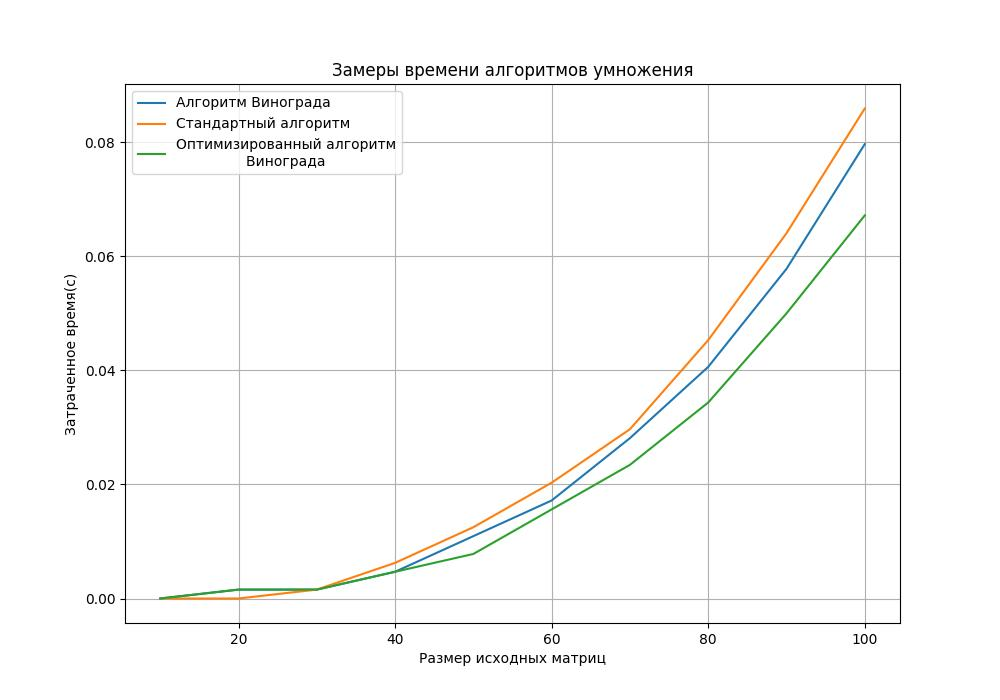
\includegraphics[scale=0.5]{img/odd.jpeg}
	\end{center}
	\captionsetup{justification=centering}
	\caption{Сравнение по времени алгоритмов умножения матриц нечетного размера}
	\label{img:odd}
\end{figure}

\section{Вывод}

В результате эксперимента было получено, что при размере матриц, большем 30, оптимизированный алгоритм Винограда работает работает быстрее стандартного алгоритма в 1.3 раза. При этом стандартный алгоритм медленнее алгоритма Винограда в 1.15 раза. Тогда, для размера матриц, начиная с 30 элементов, небходимо использовать оптимизированный алгоритм умножения матриц по Винограду.

Также в результате эксперимента было установлено, что при четном размере матриц, алгоритм Винограда работает быстрее, чем на матрицах с нечетным размером в 1.2 раза в связи с проведением дополнительных вычислений для крайних строк и столбцов. Можно сделать вывод, что алгоритм Винограда предпочтительно использовать для умножения матриц четных размеров.